\documentclass[conference]{IEEEtran}

% =========================
% Packages (IEEE-friendly)
% =========================
\usepackage{cite}
\usepackage{url}
\usepackage{amsmath,amssymb,amsfonts}
\usepackage{algorithm}
\usepackage{algorithmic}
\usepackage{graphicx}
\usepackage{textcomp}
\usepackage{xcolor}
\usepackage{array}
\usepackage{makecell}
\usepackage{booktabs}
\usepackage{multirow}
\usepackage{subcaption}
\usepackage[hidelinks]{hyperref}
\usepackage{balance} % optional: balance last page columns

\def\BibTeX{{\rm B\kern-.05em{\sc i\kern-.025em b}\kern-.08em
    T\kern-.1667em\lower.7ex\hbox{E}\kern-.125emX}}

% =========================
% Title / Authors
% =========================
% \title{Activity-Based Dwell Potential and Neutralized  Clustering
% for Urban EV Fast-Charging Planning}
\title{From Dwell Potential to Planning Districts: A Three-Stage Framework for Urban EV Fast-Charging Planning}
\author{
\IEEEauthorblockN{Ehsan Sobhani}
\IEEEauthorblockA{
Department of Electrical Engineering and Computer Science\\
York University\\
Toronto, Canada\\
ehsan666@yorku.ca}
\and
\IEEEauthorblockN{Hany E. Z. Farag}
\IEEEauthorblockA{
Department of Electrical Engineering and Computer Science\\
York University\\
Toronto, Canada\\
hefarag@yorku.ca}
}

\begin{document}
\maketitle

% =========================
% Abstract / Keywords
% =========================
\begin{abstract}
Urban EV fast-charging planning requires identifying locations where vehicles
naturally dwell long enough to charge and organizing these locations into
stable meso-scale planning regions. This paper introduces a two-layer
behavioral-to-structural framework. First, we define an \emph{Activity-Based
Dwell Potential} (ABDP) metric derived from point-of-interest (POI) categories
weighted by dwell-time compatibility with fast charging (20-40 minutes).
Second, we propose a \emph{Neutralization-Based Zonal Clustering} (NBZC) algorithm that aggregates arterial zones into contiguous, compact corridor
regions whose cluster-level imbalance between BEV density and ABDP is
approximately neutralized. A Toronto case study over 234 arterial zones shows
that ABDP is strongly associated with normalized BEV density and exhibits
significant spatial co-structure. NBZC then compresses the zone graph into a
meso-scale cluster graph while preserving connectivity and improving cohesion.
The resulting corridor-aligned regions provide a practical foundation for
charger allocation and corridor-level evaluation.
\end{abstract}

\begin{IEEEkeywords}
EV fast charging, activity-based dwell potential, spatial regionalization,
graph clustering, contiguity, compactness, corridor planning
\end{IEEEkeywords}

% =========================
% 1. Introduction
% =========================
\section{Introduction}
Fast-charging (FC) planning requires spatial units that align with how charging
opportunities arise: vehicles charge while parked, and parking durations are
driven by nearby activities. Mobility-only indicators (traffic flow, BEV density)
capture where vehicles move, but do not explicitly encode where vehicles dwell
long enough to fast charge. Conversely, very fine spatial units can exhibit
strong local mismatch between BEV density and dwell compatibility, leading to
fragmented and unstable planning decisions.

This paper proposes a two-layer framework:
(i) a behavioral signal layer using \emph{Activity-Based Dwell Potential} (ABDP),
and (ii) a structural regionalization layer using \emph{Neutralization-Based Zonal
Clustering} (NBZC) to form contiguous, compact corridor regions that
approximately neutralize BEV-ABDP imbalance.

\subsection{Contributions}
\begin{itemize}
  \item A dwell-compatible ABDP metric that reframes POIs as behavioral signals.
  \item Empirical and spatial association analysis linking ABDP to BEV density.
  \item NBZC: a shape-constrained, contiguity-preserving clustering algorithm
  that forms meso-scale corridor regions with EV-ABDP neutralization.
\end{itemize}

\section{Literature Review}

\subsection{Evolution of EV Charging Infrastructure Planning}

Early research on electric vehicle (EV) fast-charging infrastructure planning primarily emphasized grid constraints, power distribution capacity, and capital cost minimization. Demand was typically treated as an exogenous and spatially aggregated variable derived from traffic volumes, vehicle ownership statistics, or population density.\cite{BIAN2022} These infrastructure-centric models focused on network coverage and investment efficiency, with limited consideration of behavioral charging patterns.

Recent studies demonstrate a transition toward user-centric planning paradigms, where infrastructure deployment increasingly reflects mobility behavior and user convenience. Data-driven approaches incorporating heterogeneous datasets—such as traffic trajectories, land-use characteristics, and socio-economic indicators—have become prevalent. Although this shift improves spatial responsiveness to demand, most models still infer charging needs from mobility intensity rather than activity-specific behavioral dynamics.

\subsection{POI-Based Demand Modeling}

Point-of-Interest (POI) data have become a primary proxy for estimating spatial charging demand. Prior studies employ POIs to classify functional urban zones and identify potential charging hotspots using techniques such as kernel density estimation, K-Means clustering, DBSCAN clustering, location entropy analysis, and Geographic Weighted Regression (GWR).

Empirical evidence consistently shows strong correlations between certain POI categories, such as commercial centers, educational institutions, and medical facilities, and charging station distribution. However, POIs are predominantly treated as spatial demand intensifiers rather than behavioral anchors. The temporal dimension of user activities, particularly dwell duration compatibility with fast-charging session requirements, remains largely unmodeled. Consequently, existing POI-based frameworks identify \emph{where} users concentrate but do not explicitly evaluate whether the duration of their activities naturally supports fast charging.

\subsection{Machine Learning and Graph-Based Approaches}

To capture nonlinear spatial relationships and network dependencies, recent research has adopted advanced machine learning and graph-based methodologies. Support Vector Regression (SVR), multi-view Graph Convolutional Networks (GCNs), and topology-informed graph models have demonstrated improved predictive performance for charging demand estimation.

In parallel, multi-objective optimization frameworks—including evolutionary algorithms and Deep Reinforcement Learning (DRL)—have been developed to balance cost, coverage, accessibility, and fairness objectives. These methods enhance spatial intelligence and network-level optimization performance.

Despite these advancements, urban zones are typically modeled as graph nodes associated with scalar demand values. While spatial topology and connectivity are explicitly represented, behavioral feasibility—specifically the alignment between natural dwell time and required charging duration—is abstracted away. As a result, current models capture spatial accessibility but do not evaluate temporal compatibility.

\subsection{Behavioral and Structural Gap}

A limited number of studies acknowledge the temporal dimension of charging behavior by categorizing POIs according to visit duration or incorporating competition-aware demand metrics. However, these contributions remain largely descriptive and are not structurally embedded within spatial regionalization or optimization processes.

Furthermore, prevailing zoning approaches rely on predefined spatial units such as Traffic Analysis Zones (TAZs), administrative districts, or uniform grid cells. These externally imposed partitions do not necessarily reflect corridor-based mobility structures or behavioral self-sufficiency within urban regions.

Accordingly, a fundamental gap persists in the literature: the absence of a meso-scale planning framework that quantitatively integrates activity-driven dwell compatibility into endogenous regionalization and charging infrastructure planning.

\subsection{Positioning of the Proposed Framework}

To address this limitation, this study introduces \emph{Activity-Based Dwell Potential (ABDP)} as a behavioral metric that transforms POI composition into a continuous dwell-compatibility signal aligned with the temporal requirements of fast charging. Unlike prior POI-based approaches that treat urban features as static demand proxies, ABDP operationalizes the temporal feasibility of charging within specific activity contexts.

Building upon ABDP, a \emph{Neutralization-Based Zonal Clustering (NBZC)} mechanism is proposed to aggregate arterial zones into contiguous and compact corridor-based regions while minimizing the mismatch between normalized dwell potential and normalized EV density. This process produces endogenous meso-scale regions characterized by behavioral self-sufficiency.

In contrast to existing methods that focus primarily on optimal site selection within fixed spatial boundaries, the proposed framework restructures the urban system to internalize dwell--demand balance. This behavior-to-structure transformation bridges spatial network modeling, behavioral analysis, and infrastructure planning, thereby addressing a critical gap in contemporary EV charging research.
% =========================
% 2. Data and Notation
% =========================
\section{Data and Notation}

\subsection{Urban Arterial Zones}

Let the study area be partitioned into a finite collection of arterial
zones representing contiguous segments of the urban corridor network:
\begin{equation}
\mathcal{Z}^{\mathrm{Ar}} =
\{ Z^{\mathrm{Ar}}_j \subset \mathbb{R}^2 : j \in \mathcal{J} \},
\end{equation}
where $\mathcal{J}$ is the index set of zones and
$|\mathcal{J}| = N_{\mathrm{Ar}}$ denotes the total number of arterial
zones. Each $Z^{\mathrm{Ar}}_j$ is a planar polygon aligned with the
urban arterial structure and constructed such that zones are mutually
non-overlapping and collectively exhaust the study region.

The area of each zone is defined as
\begin{equation}
A^{\mathrm{Ar}}_j =
\mathrm{Area}(Z^{\mathrm{Ar}}_j), \qquad j\in\mathcal{J},
\end{equation}
with $A^{\mathrm{Ar}}_j > 0$ for all $j$. These spatial units form the
fundamental resolution at which both mobility intensity and
activity-based dwell characteristics are measured.

\subsection{BEV Density}

Let $EVC^{\mathrm{Ar}}_j$ denote the EV
count or an empirically derived EV intensity proxy associated with
zone $j$. To obtain an areal measure independent of zone size, EV density is defined as
\begin{equation}
\rho^{\mathrm{Ar}}_j =
\frac{EVC^{\mathrm{Ar}}_j}{A^{\mathrm{Ar}}_j}.
\end{equation}

Because raw density values may vary substantially across zones and are
scale-dependent, we normalize them using min--max scaling:
\begin{equation}
S^{\mathrm{EV}}_j =
\frac{\rho^{\mathrm{Ar}}_j -
\min_{k\in\mathcal{J}} \rho^{\mathrm{Ar}}_k}
{\max_{k\in\mathcal{J}} \rho^{\mathrm{Ar}}_k -
\min_{k\in\mathcal{J}} \rho^{\mathrm{Ar}}_k},
\qquad S^{\mathrm{BEV}}_j\in[0,1].
\end{equation}

The normalized quantity $S^{\mathrm{EV}}_j$ represents the relative
mobility intensity of zone $j$ within the study area. It is interpreted
as a comparative measure rather than an absolute predictor of charging
demand, thereby enabling consistent integration with normalized
behavioral indicators.

\subsection{POIs and Zone Assignment}

Let $\mathcal{P}$ denote the set of points of interest (POIs) observed
within the study region. Each POI $p\in\mathcal{P}$ is associated with
geographic coordinates $\mathbf{x}_p \in \mathbb{R}^2$ and a semantic
activity classification.

To spatially aggregate activity information, POIs are assigned to
arterial zones via the mapping
\begin{equation}
\phi : \mathcal{P}\rightarrow\mathcal{J}, \qquad
\phi(p)=j \;\text{if}\; \mathbf{x}_p\in Z^{\mathrm{Ar}}_j,
\end{equation}
which ensures that each POI is uniquely associated with exactly one
arterial zone. Based on this assignment, the set of POIs contained in
zone $j$ is defined as
\begin{equation}
\mathcal{P}_j =
\{p\in\mathcal{P}:\phi(p)=j\}.
\end{equation}

This construction enables activity-based attributes to be aggregated
consistently at the same spatial resolution as EV density.

\subsection{Adjacency Graph}

Spatial contiguity among arterial zones is represented through an
undirected adjacency graph
\[
G = (V,E),
\]
where each node $i \in V$ corresponds to arterial zone
$Z^{\mathrm{Ar}}_i$. An edge $(i,k)\in E$ exists if and only if zones
$i$ and $k$ share a boundary segment of positive length under rook
contiguity.
The set of rook neighbors of zone $i$ is denoted by
\[
N(i) = \{ k \in \mathcal{J} : (i,k)\in E \}.
\]

The graph $G$ encodes the topological structure of the arterial
network and constrains all subsequent clustering operations to produce
spatially contiguous regions. This adjacency structure ensures that
regionalization respects the geometric and functional continuity of
urban corridors.% =========================
% 3. Activity-Based Dwell Potential (ABDP)
% =========================
\section{Activity-Based Dwell Potential Modeling}

\subsection{POI Activity Classes and Dwell Times}

Urban activities generate heterogeneous visit durations that directly
influence the behavioral feasibility of fast charging. Let activity
categories be indexed by $k\in\mathcal{K}$, where each category
represents a semantically coherent group of POIs (e.g., food service,
retail, services, leisure). Each category is assigned a representative
dwell time $T_k$, reflecting the typical visit duration associated with that activity type.
The dwell time parameter $T_k$ is interpreted as the expected time a
vehicle remains parked while its user engages in the corresponding
activity. These representative values may be derived from empirical
surveys, mobility studies, domain literature, or aggregated behavioral
observations.

For arterial zone $j\in\mathcal{J}$, let $N_{jk}$ denote the number of POIs of category $k$ located within that zone.
Thus, the pair $(N_{jk}, T_k)$ jointly captures both the intensity and
the behavioral duration characteristics of activities occurring in
zone $j$.

\subsection{Dwell-Time Weighting}

Fast charging is behaviorally viable only if vehicle dwell duration
approximately matches charging session length. Let $T^\ast$ denote the
target charging-compatible dwell duration. In typical DC fast-charging
contexts, $T^\ast$ is selected near 30 minutes to reflect the
20--40 minute operational window of high-power charging.
To measure compatibility between activity dwell duration and charging
requirements, define the dwell-compatibility weight
\begin{equation}
w_k =
\exp\!\left(
-\frac{(T_k - T^\ast)^2}{2\sigma^2}
\right),
\end{equation}
where $\sigma > 0$ controls the tolerance width of the compatibility
window.

This Gaussian kernel assigns maximal weight to activity categories
whose representative dwell time equals $T^\ast$, while progressively
down-weighting activities with substantially shorter or longer
durations. The parameter $\sigma$ determines how strictly charging
feasibility is enforced: small $\sigma$ emphasizes narrow
compatibility, whereas larger $\sigma$ allows broader behavioral
alignment. Importantly, this weighting mechanism operationalizes behavioral
feasibility as a continuous function rather than a binary threshold,
thereby avoiding the arbitrary classification of activities as either
compatible or incompatible.

\subsection{Zone-Level ABDP}

The raw activity-based dwell potential for arterial zone $j$ is
defined as
\begin{equation}
S^{\mathrm{act}}_j =
\sum_{k\in\mathcal{K}} w_k\, N_{jk}.
\end{equation}

This expression integrates two dimensions simultaneously:

\begin{enumerate}
\item \emph{Activity intensity} through $N_{jk}$, and
\item \emph{Charging-duration compatibility} through $w_k$.
\end{enumerate}

Thus, $S^{\mathrm{act}}_j$ represents the aggregate charging-feasible
activity mass within zone $j$.

Because arterial zones may differ in geographic size, direct comparison
of $S^{\mathrm{act}}_j$ across zones could introduce scale bias.
Therefore, the dwell potential is normalized by zone area:
\begin{equation}
D_j =
\frac{S^{\mathrm{act}}_j}{A^{\mathrm{Ar}}_j}.
\end{equation}

The quantity $D_j$ can be interpreted as a dwell-compatible activity
density, reflecting how strongly a zone structurally supports
charging-aligned behavior per unit area.
Finally, to enable comparability with normalized EV density and to
produce a scale-independent behavioral signal, min-max normalization
is applied:
\begin{equation}
\bar{D}_j =
\frac{D_j - \min_{k\in\mathcal{J}} D_k}
{\max_{k\in\mathcal{J}} D_k - \min_{k\in\mathcal{J}} D_k},
\qquad \bar{D}_j\in[0,1].
\end{equation}

The resulting $\bar{D}_j$ constitutes the
\emph{Activity-Based Dwell Potential (ABDP)} score of zone $j$.
This metric quantifies the relative behavioral suitability of each
arterial zone for fast-charging deployment independent of observed
vehicle density.
Conceptually, ABDP captures where vehicles are \emph{likely to remain}
long enough to charge, rather than where vehicles merely pass through.
It therefore represents a behavioral complement to mobility-based
intensity measures and provides a structurally grounded foundation for
subsequent neutralization and clustering analysis.
% =========================
% 4. Empirical Relationship + Spatial Association
% =========================
% \section{Empirical Relationship and Spatial Association}
% \subsection{Global Association}
% Compute Pearson correlation between $S^{\mathrm{BEV}}_j$ and $\bar{D}_j$:
% \begin{equation}
% r =
% \frac{
% \sum_{j \in \mathcal{J}}
% \left( S^{\mathrm{BEV}}_j - \mu_{\mathrm{BEV}} \right)
% \left( \bar{D}_j - \mu_{D} \right)
% }{
% \sqrt{\sum_{j \in \mathcal{J}} \left( S^{\mathrm{BEV}}_j - \mu_{\mathrm{BEV}} \right)^2}
% \sqrt{\sum_{j \in \mathcal{J}} \left( \bar{D}_j - \mu_{D} \right)^2}
% }.
% \end{equation}

% \subsection{Bivariate Moran's $I$}
% Let $W=[w_{jk}]$ be adjacency weights ($w_{jk}=1$ if adjacent, else 0). Define:
% \begin{equation}
% I =
% \frac{|\mathcal{J}|}{\sum_{j}\sum_{k} w_{jk}}
% \,
% \frac{
% \sum_{j}\sum_{k} w_{jk}
% \left( S^{\mathrm{BEV}}_j - \mu_{\mathrm{BEV}} \right)
% \left( \bar{D}_k - \mu_{D} \right)
% }{
% \sum_{j}
% \left( S^{\mathrm{BEV}}_j - \mu_{\mathrm{BEV}} \right)^2
% }.
% \end{equation}

% =========================
% 5. Bridge: Signal -> Regionalization
% =========================
\section{From Behavioral Signal to Meso-Scale Regionalization}

While ABDP provides a behaviorally grounded diagnostic signal at the
arterial-zone level, infrastructure planning and resource allocation
are rarely executed at such fine spatial resolution. Charging
infrastructure, grid reinforcement, and corridor-level investments
are typically designed at meso-scale units that aggregate multiple
zones into coherent planning regions. Consequently, a transformation
is required from zone-level behavioral indicators to structurally
stable regional units. We therefore aggregate arterial zones into
contiguous and geometrically compact regions that
approximately neutralize EV-ABDP imbalance.

The concept of neutralization extends beyond mathematical balancing;
it is grounded in planning logic. At the arterial-zone scale, the
imbalance
\begin{equation}
d_i = \bar{D}_i - S_i^{\mathrm{EV}}
\end{equation}
quantifies the divergence between behavioral dwell compatibility and observed EV concentration. Large positive values indicate corridors
rich in dwell-compatible activities but relatively weak in EV presence, suggesting potential behavioral suitability without corresponding demand intensity. Conversely, large negative values identify zones with substantial EV density but limited dwell
compatibility, implying that vehicles may traverse these corridor zones
without remaining long enough to charge efficiently.

Planning decisions based exclusively on either signal introduce systematic bias. Allocation driven primarily by ABDP may oversupply
areas that are behaviorally compatible but insufficiently demanded.
Allocation driven primarily by EV density may place chargers in
high-mobility corridors where vehicles lack sufficient stationary
time, leading to suboptimal utilization. Neutralization addresses
this structural tension by aggregating adjacent zones with opposing imbalances so that positive and negative deviations offset at the cluster level. In doing so, the resulting region reflects co-location
of behavioral feasibility and mobility intensity rather than dominance of one over the other.

% Neutralization also contributes to stability in planning units. Individual arterial zones are sensitive to localized anomalies, such
% as a single commercial anchor, institutional facility, or transit
% node. Small perturbations in data can therefore produce large shifts in zone-level prioritization. By enforcing the condition
% \begin{equation}
%     \left| \sum_{i \in C} d_i \right| \approx 0,
% \end{equation}
% clusters represent mesoscale regions in which behavioral and mobility signals are jointly supported across multiple contiguous zones.
% Aggregation reduces sensitivity to microscale volatility and produces planning regions that are less dependent on isolated activity spikes.
% This improves robustness in long-term infrastructure decisions.
From a planning perspective, infrastructure regions should ideally be
internally self-consistent rather than structurally dependent on adjacent
areas. Regions whose charging viability relies on spillover EV demand
from neighboring zones, or whose utilization depends on exporting demand
outward, introduce instability and complicate allocation decisions.

Consider a cluster $C \subseteq \mathcal{J}$ with aggregate imbalance
\begin{equation}
\sum_{i\in C} d_i.
\end{equation}

If
\begin{equation}
\sum_{i\in C} d_i > 0,
\end{equation} 
the cluster exhibits excess dwell-compatible activity relative to EV
presence. In this case, its charging utilization depends on attracting
EVs from neighboring clusters to compensate for insufficient internal vehicle density.

Conversely, if
\begin{equation}
\sum_{i\in C} d_i < 0,
\end{equation}
the cluster exhibits excess EV intensity relative to dwell compatibility. Its charging feasibility, therefore, depends on exporting
charging behavior to adjacent regions where dwell-compatible activities are more abundant.
Both situations imply inter-regional dependency, meaning that charging
viability is not structurally supported within the region itself but relies on cross-boundary behavioral flows.

Planners generally prefer regions satisfying
\begin{equation}
\left|\sum_{i\in C} d_i\right| \approx 0,
\end{equation}
as such, regions are internally balanced and less dependent on external spillover. This condition promotes planning stability, reduces
allocation bias, and aligns infrastructure deployment with regions where mobility intensity and behavioral dwell compatibility
coexist structurally.
From an operational perspective, fast-charging feasibility requires simultaneous satisfaction of two necessary conditions: vehicles must
be present in sufficient density, and vehicles must remain stationary for durations compatible with charging. These conditions correspond, respectively, to mobility intensity and dwell compatibility. The neutralization constraint embeds both conditions into the regional
definition itself. Instead of optimizing infrastructure placement in
a post hoc manner, the regionalization process ensures that supply allocation occurs within structurally balanced environments where both determinants coexist.

% Furthermore, infrastructure deployment, transformer sizing, and distribution grid coordination are rarely performed at the scale of individual micro-zones. Utilities and municipalities operate at
% corridor or district scales that must be contiguous, interpretable, and spatially coherent. Neutralized clusters satisfy these structural requirements by preserving arterial adjacency, maintaining network
% connectivity, and enforcing geometric compactness. The compactness constraint prevents the formation of elongated or fragmented regions that would be impractical for grid integration or corridor-level
% investment planning.
% In the absence of geometric control, minimizing imbalance alone could produce snake-like chains linking distant positive and negative
% zones. Such shapes may satisfy algebraic neutrality but lack functional plausibility. By coupling imbalance minimization with a
% shape constraint, the regionalization process ensures that behavioral
% balancing occurs within spatially interpretable and deployable corridor units.

% In planning terms, neutralization performs three interconnected functions. First, it mitigates allocation bias by preventing
% systematic over-supply or under-supply driven by a single signal dominance. Second, it enforces behavioral alignment by embedding both
% mobility and dwell feasibility within each planning region. Third, it simplifies spatial structure by transforming noisy, heterogeneous
% zone-level data into units compatible with infrastructure design and grid coordination.
% Neutralization should therefore be understood not as a clustering artifact, but as a planning consistency constraint that reconciles behavioral feasibility and mobility intensity within structurally coherent urban regions.
% =========================
% 6. NBZC Clustering
% =========================
\section{Neutralization-Based Zonal Clustering With Shape Constraints}

The ABDP provides a behavioral signal
at the arterial-zone level. However, infrastructure planning and grid
allocation are rarely performed at such fine spatial resolution.
Instead, planners operate at meso-scale corridor or district levels.
Accordingly, we introduce a clustering framework that aggregates arterial zones into contiguous regions while explicitly enforcing behavioral-mobility balance. The guiding principle of this regionalization is \emph{neutralization}: clusters are formed so that excess behavioral
potential (ABDP) and excess mobility intensity (BEV density) offset each other at the cluster level, thereby reducing systematic over-supply or under-supply bias.

% \subsection{Zone-Level Imbalance}

% Let $S_i^{\mathrm{BEV}}$ denote normalized BEV density and
% $\bar{D}_i$ denote normalized ABDP in zone $i$. We define the
% zone-level imbalance as
% \begin{equation}
% d_i = \bar{D}_i - S_i^{\mathrm{BEV}}.
% \label{eq:di}
% \end{equation}

% The quantity $d_i$ measures the directional mismatch between
% behavioral dwell compatibility and observed EV concentration:

% \begin{itemize}
% \item $d_i > 0$: behavioral dwell capacity exceeds EV intensity,
%       indicating potential under-utilization risk if chargers are
%       allocated solely by activity.
% \item $d_i < 0$: EV intensity exceeds dwell compatibility,
%       indicating feasibility risk if chargers are allocated solely
%       by mobility.
% \end{itemize}

% Neutralization seeks to combine adjacent zones such that these
% imbalances cancel at the cluster level.

\subsection{Neutralization Objective}

For a cluster $C \subseteq V$ and candidate addition $j$,
define the absolute cluster imbalance as
\begin{equation}
\mathrm{imb}(C\cup\{j\}) =
\left|\sum_{i\in C\cup\{j\}} d_i\right|.
\label{eq:imb}
\end{equation}

Minimizing \eqref{eq:imb} enforces approximate balance between
ABDP and EV intensity at the aggregated level. Importantly,
neutralization is not defined zone-by-zone, but at the cluster
level, reflecting the reality that infrastructure deployment
operates over corridor-scale regions.

\subsection{Compactness Proxy}

Neutralization alone is insufficient because imbalance cancellation
could occur between distant zones, producing elongated or
non-interpretable clusters. To preserve geometric coherence, we
introduce a compactness constraint.

Let each zone have centroid $\mathbf{x}_i\in\mathbb{R}^2$
in a projected metric coordinate system. The centroid of cluster $C$
is
\begin{equation}
\bar{\mathbf{x}}_{C} =
\frac{1}{|C|}\sum_{i\in C}\mathbf{x}_i,
\end{equation}
and define the radius-based compactness measure
\begin{equation}
r(C) =
\max_{i\in C}
\left\|
\mathbf{x}_i - \bar{\mathbf{x}}_{C}
\right\|.
\label{eq:radius}
\end{equation}

The radius $r(C)$ measures the maximum dispersion of zones within the
cluster. Smaller values correspond to more compact regions. This proxy prevents the formation of snake-like chains that would satisfy neutralization algebraically but violate spatial
coherence.

\subsection{Combined Score}

To balance behavioral neutralization and geometric compactness,
candidate zone $j$ is evaluated using
\begin{equation}
\mathrm{score}(C\cup\{j\}) =
\left|\sum_{i\in C\cup\{j\}} d_i\right|
+\lambda_{\mathrm{shape}}\,
r(C\cup\{j\}),
\label{eq:score}
\end{equation}
where $\lambda_{\mathrm{shape}}\ge 0$ controls the trade-off between
imbalance reduction and shape regularity.

When $\lambda_{\mathrm{shape}}=0$, clustering prioritizes purely
behavioral neutralization. Increasing $\lambda_{\mathrm{shape}}$
tightens geometric cohesion and prevents spatial overextension.
Thus, \eqref{eq:score} operationalizes a multi-objective balance
between functional alignment and spatial feasibility.

\subsection{Greedy Frontier Growth}

Let $U$ denote the set of unassigned zones. Clusters are constructed
sequentially using a greedy frontier expansion strategy.
Each cluster is seeded from the unassigned zone with largest
absolute imbalance:
\[
i^*=\arg\max_{i\in U}|d_i|.
\]

Seeding at high-magnitude imbalance ensures that extreme zones,
which are most structurally mismatched, are neutralized first.
Given current cluster $C$, the candidate frontier is
\begin{equation}
F =
\Big(
\bigcup_{i\in C} N(i)
\Big)\cap U,
\end{equation}
where $N(i)$ denotes rook-adjacent neighbors. This guarantees that
clusters remain spatially contiguous at every growth step.

Among candidates in $F$, the algorithm selects
\[
j^*=\arg\min_{j\in F}
\mathrm{score}(C\cup\{j\})
\]
subject to stopping rules described below.

\subsection{Stopping Rules}

Cluster growth terminates when any of the following conditions holds:

\begin{itemize}
  \item \textbf{Size cap:} $|C|\geq \texttt{max\_cluster\_size}$,
        preventing excessively large aggregation.
  \item \textbf{Imbalance cap:} adding the best candidate violates
        $\mathrm{imb}(C\cup\{j\})>
        \texttt{max\_abs\_imbalance}$,
        ensuring bounded residual mismatch.
  \item \textbf{Shape cap:} candidate exceeds
        $r(C\cup\{j\})>
        \texttt{max\_radius}$,
        preserving compact geometry.
  \item \textbf{Neutralization safeguard:}
        if $|C|\ge 2$ and any addition increases
        $\left|\sum_{i\in C} d_i\right|$,
        growth halts to avoid deterioration of balance.
\end{itemize}

These constraints jointly ensure that clusters remain
behaviorally balanced, spatially contiguous, geometrically compact,
and bounded in scale.

\begin{algorithm}[t]
\caption{NBZC: Greedy Neutralization + Shape-Constrained Clustering}
\label{alg:nbzc}
\begin{algorithmic}[1]
\STATE \textbf{Input:} graph $G=(V,E)$, $S_i^{\mathrm{BEV}}$, $\bar{D}_i$,
centroids $\mathbf{x}_i$, $\lambda_{\mathrm{shape}}$,
\texttt{max\_cluster\_size}, \texttt{max\_abs\_imbalance}, \texttt{max\_radius}
\STATE Compute $d_i\leftarrow \bar{D}_i - S_i^{\mathrm{BEV}}$
\STATE $U \leftarrow V$, $\mathcal{C}\leftarrow \emptyset$
\WHILE{$U\neq \emptyset$}
  \STATE $i^*\leftarrow \arg\max_{i\in U}|d_i|$; $C\leftarrow\{i^*\}$; $U\leftarrow U\setminus\{i^*\}$
  \WHILE{true}
    \STATE $F\leftarrow \left(\bigcup_{i\in C}N(i)\right)\cap U$
    \IF{$F=\emptyset$} \STATE \textbf{break} \ENDIF
    \STATE Choose $j^*\in F$ minimizing $\mathrm{score}(C\cup\{j\})$ in \eqref{eq:score}
    \IF{$|C|\ge \texttt{max\_cluster\_size}$} \STATE \textbf{break} \ENDIF
    \IF{$\mathrm{imb}(C\cup\{j^*\})>\texttt{max\_abs\_imbalance}$} \STATE \textbf{break} \ENDIF
    \IF{$r(C\cup\{j^*\})>\texttt{max\_radius}$} \STATE \textbf{break} \ENDIF
    \IF{$|C|\ge 2$ \AND $\left|\sum_{i\in C}d_i\right|<
        \left|\sum_{i\in C\cup\{j^*\}}d_i\right|$}
      \STATE \textbf{break}
    \ENDIF
    \STATE $C\leftarrow C\cup\{j^*\}$; $U\leftarrow U\setminus\{j^*\}$
  \ENDWHILE
  \STATE $\mathcal{C}\leftarrow \mathcal{C}\cup\{C\}$
\ENDWHILE
\STATE \textbf{Output:} clusters $\mathcal{C}$
\end{algorithmic}
\end{algorithm}

This procedure produces a partition of the arterial zones network into
meso-scale regions that (i) remain contiguous under rook adjacency,
(ii) approximately neutralize ABDP–BEV imbalance, and
(iii) satisfy geometric compactness constraints.
% =========================
% 7. Evaluation Metrics (Meso-scale)
% =========================
\section{Evaluation Metrics}

\subsection{Cluster-Level Neutralization}

To evaluate the effectiveness of the neutralization-based regionalization,
we measure the degree to which imbalance is reduced after aggregation.
Recall that zone-level imbalance is defined as
\begin{equation}
d_i = \bar{D}_i - S_i^{\mathrm{EV}},
\end{equation}
where $\bar{D}_i$ denotes the normalized ABDP and $S_i^{\mathrm{EV}}$ denotes normalized EV density.

\subsubsection*{Cluster Imbalance}

For each cluster $c \subseteq \mathcal{J}$, define aggregate imbalance as
\begin{equation}
\Delta_c = \sum_{i\in c} d_i.
\end{equation}

The sign of $\Delta_c$ indicates structural bias:

\begin{itemize}
\item $\Delta_c > 0$: excess dwell compatibility relative to EV density.
\item $\Delta_c < 0$: excess EV density relative to dwell compatibility.
\end{itemize}
Because clusters may vary in size and signal magnitude, we define a
scale-independent neutralization index
\begin{equation}
\eta_c =
\frac{|\Delta_c|}
{\sum_{i\in c} \left(\bar{D}_i + S_i^{\mathrm{EV}}\right)}.
\label{eq:eta_c}
\end{equation}
The denominator represents the total combined signal magnitude within
cluster $c$, ensuring that imbalance is evaluated relative to the
cluster's structural scale.

By construction,
\[
0 \le \eta_c \le 1.
\]
Lower values of $\eta_c$ indicate a stronger internal balance between
behavioral dwell compatibility and mobility intensity.

\subsubsection*{Zone-Level Baseline}

To assess improvement relative to the original zoning resolution,
define the zone-level imbalance index
\begin{equation}
\eta_i =
\frac{|d_i|}
{\bar{D}_i + S_i^{\mathrm{EV}} + \epsilon},
\end{equation}
where $\epsilon>0$ is a small constant preventing division by zero.
Comparing the distributions of $\eta_i$ and $\eta_c$ quantifies the
extent to which clustering internalizes opposing imbalances.
A systematic reduction from $\eta_i$ to $\eta_c$ indicates successful
meso-scale neutralization and reduced structural dependency across
regional boundaries.

\section{Methodology: From Neutralized Clusters to Planning Districts}

Let the neutralized cluster graph be denoted as 
$G_c = (V_c, E_c)$, where each node $c \in V_c$ represents a previously derived cluster and edges encode spatial contiguity. 
Each cluster $c$ is associated with a normalized dwell signal $\bar{D}_c$, normalized EV density $S_c^{EV}$, and behavioral mismatch

\begin{equation}
d_c = \bar{D}_c - S_c^{EV}.
\label{eq:cluster_mismatch}
\end{equation}

\subsection{Community-Level Neutralization}

Let $\mathcal{G} = \{ g_1, \dots, g_k \}$ denote a partition of $V_c$ into $k$ communities (candidate planning districts). 
For a community $g \subseteq V_c$, define its aggregate mismatch:

\begin{equation}
\Delta_g = \sum_{c \in g} d_c,
\label{eq:community_mismatch}
\end{equation}

and its total signal magnitude:

\begin{equation}
T_g = \sum_{c \in g} \left( \bar{D}_c + S_c^{EV} \right).
\label{eq:community_mass}
\end{equation}

The scale-independent neutralization index for a community is defined as

\begin{equation}
\eta_g = \frac{|\Delta_g|}{T_g}.
\label{eq:eta_g}
\end{equation}

The global community neutralization objective is

\begin{equation}
J_{\text{neutral}}(k) =
\frac{\sum_{g \in \mathcal{G}} \eta_g T_g}
{\sum_{g \in \mathcal{G}} T_g}.
\label{eq:J_neutral}
\end{equation}

Lower values indicate stronger behavioral self-sufficiency.

\subsection{Exhaustive Scale Sweep}

The number of communities $k$ is swept over

\begin{equation}
k = 1, 2, \dots, |V_c|.
\label{eq:k_range}
\end{equation}

For each $k$, multiple community extraction algorithms are applied across parameter grids. 
The best achievable neutralization is recorded as

\begin{equation}
J_{\text{best}}(k) = 
\min_{\mathcal{G}: |\mathcal{G}|=k}
J_{\text{neutral}}(\mathcal{G}).
\label{eq:J_best}
\end{equation}

The curve $k \mapsto J_{\text{best}}(k)$ is analyzed to identify a stability window 
$k \in [k_{\min}, k_{\max}]$ using curvature or marginal change analysis.

\subsection{Community Extractors and Parameterization}

\subsubsection{Louvain Modularity Optimization}

Louvain maximizes modularity:

\begin{equation}
Q =
\sum_{g}
\left(
\frac{E_g}{|E|}
-
\left( \frac{\deg_g}{2|E|} \right)^2
\right),
\label{eq:modularity}
\end{equation}

where $E_g$ is the number of intra-community edges.

Resolution parameter $\gamma$ modifies the null model:

\begin{equation}
Q(\gamma) =
\sum_{g}
\left(
\frac{E_g}{|E|}
-
\gamma
\left( \frac{\deg_g}{2|E|} \right)^2
\right).
\label{eq:louvain_gamma}
\end{equation}

Parameters:
\begin{itemize}
\item Resolution $\gamma \in \Gamma$
\item Random seed $s$
\end{itemize}

\subsubsection{Asynchronous Fluid Communities}

Fluid communities partition into fixed $k$ communities by iterative label propagation under volume constraints:

\begin{equation}
\max \sum_{c \in g} \mathbb{1}(\text{majority label})
\label{eq:fluid}
\end{equation}

Parameters:
\begin{itemize}
\item Target community count $k$
\item Random seed $s$
\end{itemize}

\subsubsection{Greedy Modularity}

Hierarchical agglomeration maximizing $\Delta Q$ at each merge step.

\subsubsection{Label Propagation}

Communities evolve via majority neighbor label updates:

\begin{equation}
\ell_c^{(t+1)} = 
\arg\max_\ell |\{ c' \in \mathcal{N}(c): \ell_{c'}^{(t)} = \ell \}|.
\end{equation}

\subsubsection{Kernighan--Lin Bisection}

Two-way partition minimizing cut cost:

\begin{equation}
\min_{\mathcal{G}} \sum_{(u,v) \in E} \mathbb{1}(u \in g_1, v \in g_2).
\end{equation}

\subsection{Structural Quality Metrics}
\label{subsec:struct_metrics}

Within $[k_{\min}, k_{\max}]$, candidate partitions are evaluated using three structural metrics: coverage, modularity, and performance.

\subsubsection{Coverage}
Coverage measures the fraction of edges that lie within communities:
\begin{equation}
\mathrm{Coverage}=
\frac{\text{intra-community edges}}{|E|}.
\label{eq:coverage}
\end{equation}

\subsubsection{Modularity}
Modularity quantifies how much the observed intra-community connectivity exceeds that expected under a degree-preserving null model. For a partition $\mathcal{G}=\{g_1,\dots,g_k\}$, modularity is defined as
\begin{equation}
Q=
\frac{1}{2|E|}
\sum_{u\in V}\sum_{v\in V}
\left(
A_{uv}-\frac{k_u k_v}{2|E|}
\right)\mathbf{1}\!\left[g(u)=g(v)\right],
\label{eq:modularity}
\end{equation}
where $A_{uv}$ is the adjacency matrix of $G$, $k_u$ is the degree of node $u$, and $\mathbf{1}[\cdot]$ is the indicator function. Larger $Q$ indicates stronger community structure beyond chance.

If a resolution parameter $\gamma$ is used (e.g., Louvain), the generalized modularity becomes
\begin{equation}
Q(\gamma)=
\frac{1}{2|E|}
\sum_{u\in V}\sum_{v\in V}
\left(
A_{uv}-\gamma\frac{k_u k_v}{2|E|}
\right)\mathbf{1}\!\left[g(u)=g(v)\right].
\label{eq:modularity_gamma}
\end{equation}

\subsubsection{Performance}
Performance measures the fraction of correctly classified node pairs, counting (i) pairs placed in the same community that are connected and (ii) pairs placed in different communities that are not connected:
\begin{equation}
\mathrm{Performance}=
\frac{\text{correctly classified node pairs}}{\binom{|V|}{2}}.
\label{eq:performance}
\end{equation}
% \subsection{Pareto-Based Multi-Objective Selection}
% \label{subsec:pareto_selection}

% Within the admissible scale window $k \in [k_{\min}, k_{\max}]$, each candidate partition $\mathcal{G}$ is evaluated using the structural metric vector
% \begin{equation}
% \mathbf{s}(\mathcal{G}) =
% \big(\mathrm{Coverage}(\mathcal{G}),\, Q(\mathcal{G}),\, \mathrm{Performance}(\mathcal{G})\big),
% \label{eq:struct_vector}
% \end{equation}
% where all three components are to be \emph{maximized}. Since these objectives may conflict, we avoid scalarization and adopt Pareto efficiency.

% For two candidate partitions $\mathcal{G}_a$ and $\mathcal{G}_b$, $\mathcal{G}_a$ \emph{dominates} $\mathcal{G}_b$ (denoted $\mathcal{G}_a \succ \mathcal{G}_b$) if and only if
% \begin{equation}
% \mathrm{Coverage}(\mathcal{G}_a) \ge \mathrm{Coverage}(\mathcal{G}_b),\;
% Q(\mathcal{G}_a) \ge Q(\mathcal{G}_b),\;
% \mathrm{Performance}(\mathcal{G}_a) \ge \mathrm{Performance}(\mathcal{G}_b),
% \label{eq:pareto_dom_ge}
% \end{equation}
% and at least one inequality is strict:
% \begin{equation}
% \mathrm{Coverage}(\mathcal{G}_a) > \mathrm{Coverage}(\mathcal{G}_b)
% \;\;\text{or}\;\;
% Q(\mathcal{G}_a) > Q(\mathcal{G}_b)
% \;\;\text{or}\;\;
% \mathrm{Performance}(\mathcal{G}_a) > \mathrm{Performance}(\mathcal{G}_b).
% \label{eq:pareto_dom_strict}
% \end{equation}
% The Pareto front $\mathcal{P}^\star$ is then defined as the set of non-dominated solutions:
% \begin{equation}
% \mathcal{P}^\star =
% \left\{
% \mathcal{G} \;:\; \nexists\, \mathcal{G}' \text{ such that } \mathcal{G}' \succ \mathcal{G}
% \right\}.
% \label{eq:pareto_front}
% \end{equation}

% To preserve behavioral admissibility, we further restrict $\mathcal{P}^\star$ using the community self-balance objective $J_{\text{neutral}}(\mathcal{G})$, which is to be \emph{minimized}. Specifically, we retain only solutions in the lowest $\rho$-quantile (e.g., $\rho \in [0.1, 0.2]$) of $J_{\text{neutral}}$ values within $\mathcal{P}^\star$:
% \begin{equation}
% \mathcal{P}^\star_{\rho} =
% \left\{
% \mathcal{G} \in \mathcal{P}^\star
% \;:\;
% J_{\text{neutral}}(\mathcal{G}) \le q_{\rho}
% \right\},
% \label{eq:pareto_J_filter}
% \end{equation}
% where $q_{\rho}$ denotes the empirical $\rho$-quantile of $\{J_{\text{neutral}}(\mathcal{G}) : \mathcal{G}\in \mathcal{P}^\star\}$.

% Finally, among $\mathcal{P}^\star_{\rho}$ we select the partition that maximizes structural coherence. In our implementation, this is realized by choosing the solution that maximizes modularity $Q$ and using coverage and performance as tie-breakers:
% \begin{equation}
% \mathcal{G}^{\star} =
% \arg\max_{\mathcal{G}\in \mathcal{P}^\star_{\rho}}
% \Big( Q(\mathcal{G}),\; \mathrm{Coverage}(\mathcal{G}),\; \mathrm{Performance}(\mathcal{G}) \Big),
% \label{eq:final_selection_lex}
% \end{equation}
% where the $\arg\max$ is interpreted in lexicographic order. The maximization in (\ref{eq:final_selection_lex}) is interpreted in 
% lexicographic order. That is, candidate partitions within 
% $\mathcal{P}^\star_{\rho}$ are first compared with respect to modularity 
% $Q(\mathcal{G})$, and the solution(s) achieving the largest modularity 
% value are retained. If multiple partitions attain the same maximal 
% modularity, coverage is used as a secondary criterion to break ties. 
% Formally, let

% \begin{equation}
% \mathcal{S}_Q =
% \left\{
% \mathcal{G} \in \mathcal{P}^\star_{\rho} :
% Q(\mathcal{G}) =
% \max_{\mathcal{H} \in \mathcal{P}^\star_{\rho}} Q(\mathcal{H})
% \right\}.
% \end{equation}

% If $|\mathcal{S}_Q| > 1$, we select among them the solution that maximizes 
% coverage:

% \begin{equation}
% \mathcal{S}_{Q,C} =
% \left\{
% \mathcal{G} \in \mathcal{S}_Q :
% \mathrm{Coverage}(\mathcal{G}) =
% \max_{\mathcal{H} \in \mathcal{S}_Q} 
% \mathrm{Coverage}(\mathcal{H})
% \right\}.
% \end{equation}

% If ties persist, performance is used as the final discriminator:

% \begin{equation}
% \mathcal{G}^\star =
% \arg\max_{\mathcal{G} \in \mathcal{S}_{Q,C}}
% \mathrm{Performance}(\mathcal{G}).
% \end{equation}

% This hierarchical comparison ensures that modularity 
% dominates the selection process, while coverage and performance 
% act as progressively weaker structural refinement criteria.
\subsection{Multi-Objective Pareto and Stability Analysis}

The selection of planning district resolution was formulated as a
multi-objective evaluation problem over the number of communities $k$.
For each $k \in \{2, \dots, 130\}$, the partition achieving the minimum
$J_{\mathrm{neutralization}}$ across all algorithms and parameter
configurations was retained. Let the corresponding structural metrics be
denoted by modularity $Q(k)$, performance $P(k)$, and coverage $C(k)$.

To assess structural efficiency, we defined the objective vector
\begin{equation}
\mathbf{f}(k) =
\left(
- J_{\mathrm{neutralization}}(k),
\; Q(k),
\; P(k),
\; C(k)
\right),
\end{equation}
where $J_{\mathrm{neutral}}$ is negated so that all components
are maximized.

A community count $k_1$ is said to dominate $k_2$ if
\begin{equation}
f_i(k_1) \ge f_i(k_2) \quad \forall i,
\end{equation}
and
\begin{equation}
\exists j \text{ such that } f_j(k_1) > f_j(k_2).
\end{equation}
The Pareto regime is therefore defined as
\begin{equation}
\mathcal{K}_{\mathrm{Pareto}}
=
\left\{
k \;:\;
\text{no } k' \text{ dominates } k
\right\}.
\end{equation}

To further quantify structural robustness, a stability score was defined
based on first-order sensitivity of the normalized metrics. Let
$\tilde{M}(k)$ denote the normalized value of a metric $M \in
\{J,Q,P,C\}$. The stability of metric $M$ at resolution $k$ is computed as
\begin{equation}
S_M(k)
=
1 -
\frac{|\tilde{M}(k+1) - \tilde{M}(k)|}
{\max_{k} |\tilde{M}(k+1) - \tilde{M}(k)|}.
\end{equation}
The aggregate stability score is then defined as
\begin{equation}
S(k)
=
\frac{1}{4}
\left(
S_J(k) + S_Q(k) + S_P(k) + S_C(k)
\right).
\end{equation}
High values of $S(k)$ indicate a regime in which small variations in
community count produce minimal structural or behavioral disruption.

\subsection{Multi-Objective Pareto and Stability Analysis}

The selection of planning district resolution was formulated as a two-stage
model-selection problem over the number of communities $k$.
In Stage~1, an exhaustive $k$-sweep is used to identify a knee point
$k_{\mathrm{knee}}$ in the best-achievable neutralization curve. In Stage~2,
the final resolution is selected \emph{only within} the pre-knee regime
$k \in \{2,\dots,k_{\mathrm{knee}}\}$ using multi-objective Pareto efficiency
and a robustness (stability) criterion. The knee point therefore serves as a
search-space delimiter rather than a direct choice of $k$.

\subsubsection*{Stage 1: Exhaustive $k$-sweep and knee detection}

For each $k \in \{2,\dots,130\}$, multiple community extraction algorithms were
run over their parameter grids (and repeated across random seeds where
applicable). For each $k$, the partition achieving the minimum neutralization
objective was retained:
\begin{equation}
J_{\mathrm{best}}(k)=\min_{\mathcal{G}:|\mathcal{G}|=k} J_{\mathrm{neutral}}(\mathcal{G}).
\end{equation}
The resulting curve $k \mapsto J_{\mathrm{best}}(k)$ typically exhibits a
coarse-to-fine transition: coarse partitions (small $k$) can strongly internalize
opposing behavioral deviations, while excessive fragmentation progressively
reduces behavioral self-sufficiency.

A knee point $k_{\mathrm{knee}}$ is identified on $J_{\mathrm{best}}(k)$ using a
curvature-based criterion (e.g., maximum deviation from a chord connecting the
endpoints in the normalized $(k, J_{\mathrm{best}}(k))$ plane). This knee marks
the transition between a strongly aggregative regime and the onset of a
stabilized behavioral regime. Importantly, $k_{\mathrm{knee}}$ is \emph{not} the
final answer; it only restricts subsequent selection to the admissible
pre-knee resolution set:
\begin{equation}
\mathcal{K}_{\mathrm{adm}}=\{2,3,\dots,k_{\mathrm{knee}}\}.
\end{equation}

\subsubsection*{Stage 2: Pareto and stability selection on $\mathcal{K}_{\mathrm{adm}}$}

For each $k \in \mathcal{K}_{\mathrm{adm}}$, let the retained best-neutralization
partition have structural metrics modularity $Q(k)$, performance $P(k)$, and
coverage $C(k)$. We define the objective vector
\begin{equation}
\mathbf{f}(k)=\left(-J_{\mathrm{best}}(k),\;Q(k),\;P(k),\;C(k)\right),
\end{equation}
where $-J_{\mathrm{best}}(k)$ is maximized so that all components are aligned
for maximization.

A community count $k_1$ is said to dominate $k_2$ if
\begin{equation}
f_i(k_1)\ge f_i(k_2)\ \forall i,
\quad\text{and}\quad
\exists j:\ f_j(k_1)>f_j(k_2).
\end{equation}
The Pareto-admissible set is then
\begin{equation}
\mathcal{K}_{\mathrm{Pareto}}
=
\left\{
k \in \mathcal{K}_{\mathrm{adm}} \;:\;
\text{no } k' \in \mathcal{K}_{\mathrm{adm}} \text{ dominates } k
\right\}.
\end{equation}

To quantify robustness with respect to small changes in resolution, we compute
a stability score using first-order sensitivity of \emph{normalized} metrics.
Let $\tilde{M}(k)$ denote the normalized value of a metric
$M \in \{J,Q,P,C\}$ over $k \in \mathcal{K}_{\mathrm{adm}}$. Metric stability is
\begin{equation}
S_M(k)=
1-
\frac{|\tilde{M}(k+1)-\tilde{M}(k)|}
{\max_{k\in\mathcal{K}_{\mathrm{adm}}}\,|\tilde{M}(k+1)-\tilde{M}(k)|},
\end{equation}
and the aggregate stability score is
\begin{equation}
S(k)=\frac{1}{4}\left(S_J(k)+S_Q(k)+S_P(k)+S_C(k)\right).
\end{equation}

Finally, the selected resolution is chosen among Pareto-efficient candidates by
maximizing robustness:
\begin{equation}
k^\star=\arg\max_{k \in \mathcal{K}_{\mathrm{Pareto}}} S(k).
\end{equation}
This ensures that $k_{\mathrm{knee}}$ is used only to bound the search space,
while the final district count emerges from a joint behavioral--structural
trade-off with explicit stability control.% =========================
% 8. Results (Placeholders)
% =========================
\section{Results}

% \subsection{Experiment Setup and Parameterization}
The proposed NBZC algorithm was evaluated on the Toronto arterial-zone system
($N_{\mathrm{Ar}}=234$). All geometric calculations used a metric coordinate
reference system to ensure distance-based shape penalties are meaningful. In
particular, arterial polygons were projected to UTM (EPSG:32617), and cluster
compactness was computed using centroid coordinates in meters.
Spatial contiguity was enforced using a rook-adjacency graph constructed from
shared polygon boundaries (binary weights). Candidate growth was restricted to
the one-hop frontier induced by this rook graph. 
% EV density and ABDP were both
% treated as normalized signals in $[0,1]$.
% using the columns
% \texttt{BEV\_density\_norm} and \texttt{S\_norm\_con}, respectively. The signed
% zone-level imbalance driving neutralization was defined as
% \begin{equation}
% d_i = \bar{D}_i - S_i^{\mathrm{BEV}}.
% \end{equation}

% NBZC was run with the following parameter values, chosen to (i) prevent
% overly large regions, (ii) limit residual within-cluster imbalance, and (iii)
% avoid elongated ``chain'' clusters:
% \begin{itemize}
% \item \textbf{Contiguity:} rook adjacency ($w_{ij}\in\{0,1\}$).
% \item \textbf{Max cluster size:} $\texttt{max\_cluster\_size}=15$ zones.
% \item \textbf{Imbalance tolerance:} $\texttt{max\_abs\_imbalance}=0.5$.
% \item \textbf{Shape trade-off:} $\lambda_{\mathrm{shape}}=5\times 10^{-4}$.
% \item \textbf{Shape hard cap:} $\texttt{max\_radius}=6000$ m.
% \end{itemize}
% The combined score used during growth was
% \begin{equation}
% \mathrm{score}(C\cup\{j\}) =
% \left|\sum_{i\in C\cup\{j\}} d_i\right|
% +\lambda_{\mathrm{shape}}\, r(C\cup\{j\}),
% \end{equation}
% where $r(\cdot)$ is the maximum centroid distance to the cluster centroid
% (Euclidean, in meters). These settings emphasize neutralization while still
% penalizing spatial spread; the radius cap provides a hard safeguard against
% uninterpretable, corridor-spanning chains.
% ============================================================
% 2) Sensitivity analysis (justify selection)
% ============================================================
\subsection{Sensitivity Analysis and Parameter Selection}

To avoid dependence on an arbitrary parameter choice, a systematic sensitivity
analysis was conducted over a structured parameter grid. The maximum cluster
size was varied across small to moderate region limits: 2, 4, 8, 12, 15, and 20
zones to examine how strongly cluster size constraints influence aggregation.
The imbalance tolerance was tested at seven levels: 0.1,  0.2, 0.3, 0.5, 0.7, 0.8, and 1.0 to
evaluate how strictly within-cluster EV-ABDP mismatch is controlled.
The shape trade-off coefficient was varied from no shape penalty to
increasingly stronger penalties 0, 0.0002, 0.0005, and 0.0010 in order to assess how compactness pressure alters region geometry. Finally, an optional
hard cap on cluster radius was examined using no cap and six distance limits: none, 1000 m, 2000 m, 4000 m, 6000 m, and 8000 m to prevent excessively elongated regions.
The full factorial combination of these settings resulted in 1008 distinct
NBZC runs.
Each run was evaluated using two competing minimization objectives:
(i) total absolute cluster imbalance
$\sum_c |\Delta_c|$ and
(ii) mean cluster radius.

Fig.~\ref{fig:pareto_tradeoff} visualizes the resulting trade-off space.
Grey points correspond to all 1008 parameter combinations evaluated.
Points on the Pareto frontier (i.e., non-dominated solutions under
simultaneous minimization of neutralization loss and compactness)
are highlighted. Among these Pareto-efficient configurations, a
knee-selection criterion was applied by choosing the solution
closest to the normalized ideal corner (low imbalance and low radius).
The selected Pareto-knee configuration is explicitly indicated in
Fig.~\ref{fig:pareto_tradeoff} and the selected Pareto-knee configuration corresponds to a relatively strict
size constraint, limiting clusters to a maximum of eight zones. The imbalance
tolerance is set to 0.5, allowing moderate internal compensation between EV density and ABDP while preventing large residual mismatch. A small but
non-zero shape penalty, 0.0002, is applied, ensuring compact geometry without
overpowering the neutralization objective. In addition, a 1000 m hard cap on
cluster radius is enforced to prevent elongated corridor-spanning chains.
This operating point achieves a balanced trade-off between internal
neutralization and spatial compactness. Under this configuration,
the total absolute cluster imbalance is 8.51, while the mean cluster
radius is approximately 446 meters. The solution produces 133 clusters,
reflecting a relatively fine-grained regionalization with strong
geometric compactness. This configuration is therefore adopted for
all subsequent spatial and graph-level analyses.\begin{figure}[h]
\centering
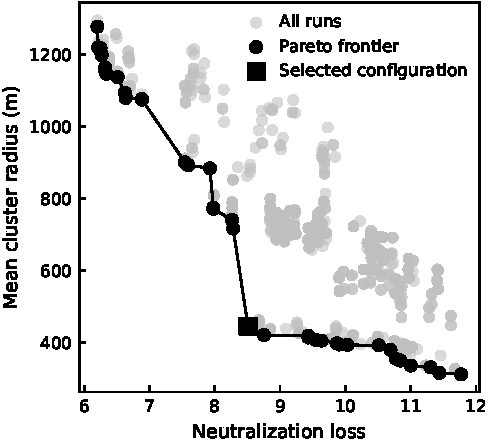
\includegraphics[width=\linewidth]{neutralization_vs_compactness_rook.pdf}
\caption{Neutralization-compactness trade-off across sensitivity runs.
}
\label{fig:pareto_tradeoff}
\end{figure}
% \subsection{Mapping and Cluster Geometry}
Fig.~\ref{fig:before_clusters} visualizes the original arterial zones. Fig.~\ref{fig:after_clusters} shows the result after dissolving polygons by cluster label, highlighting the meso-scale regional
envelopes produced by NBZC. Qualitatively, clusters remain contiguous, maintain corridor-scale interpretability, and avoid long, thin
shapes due to the radius penalty and hard cap.

% \begin{figure}[t]
% \centering
% 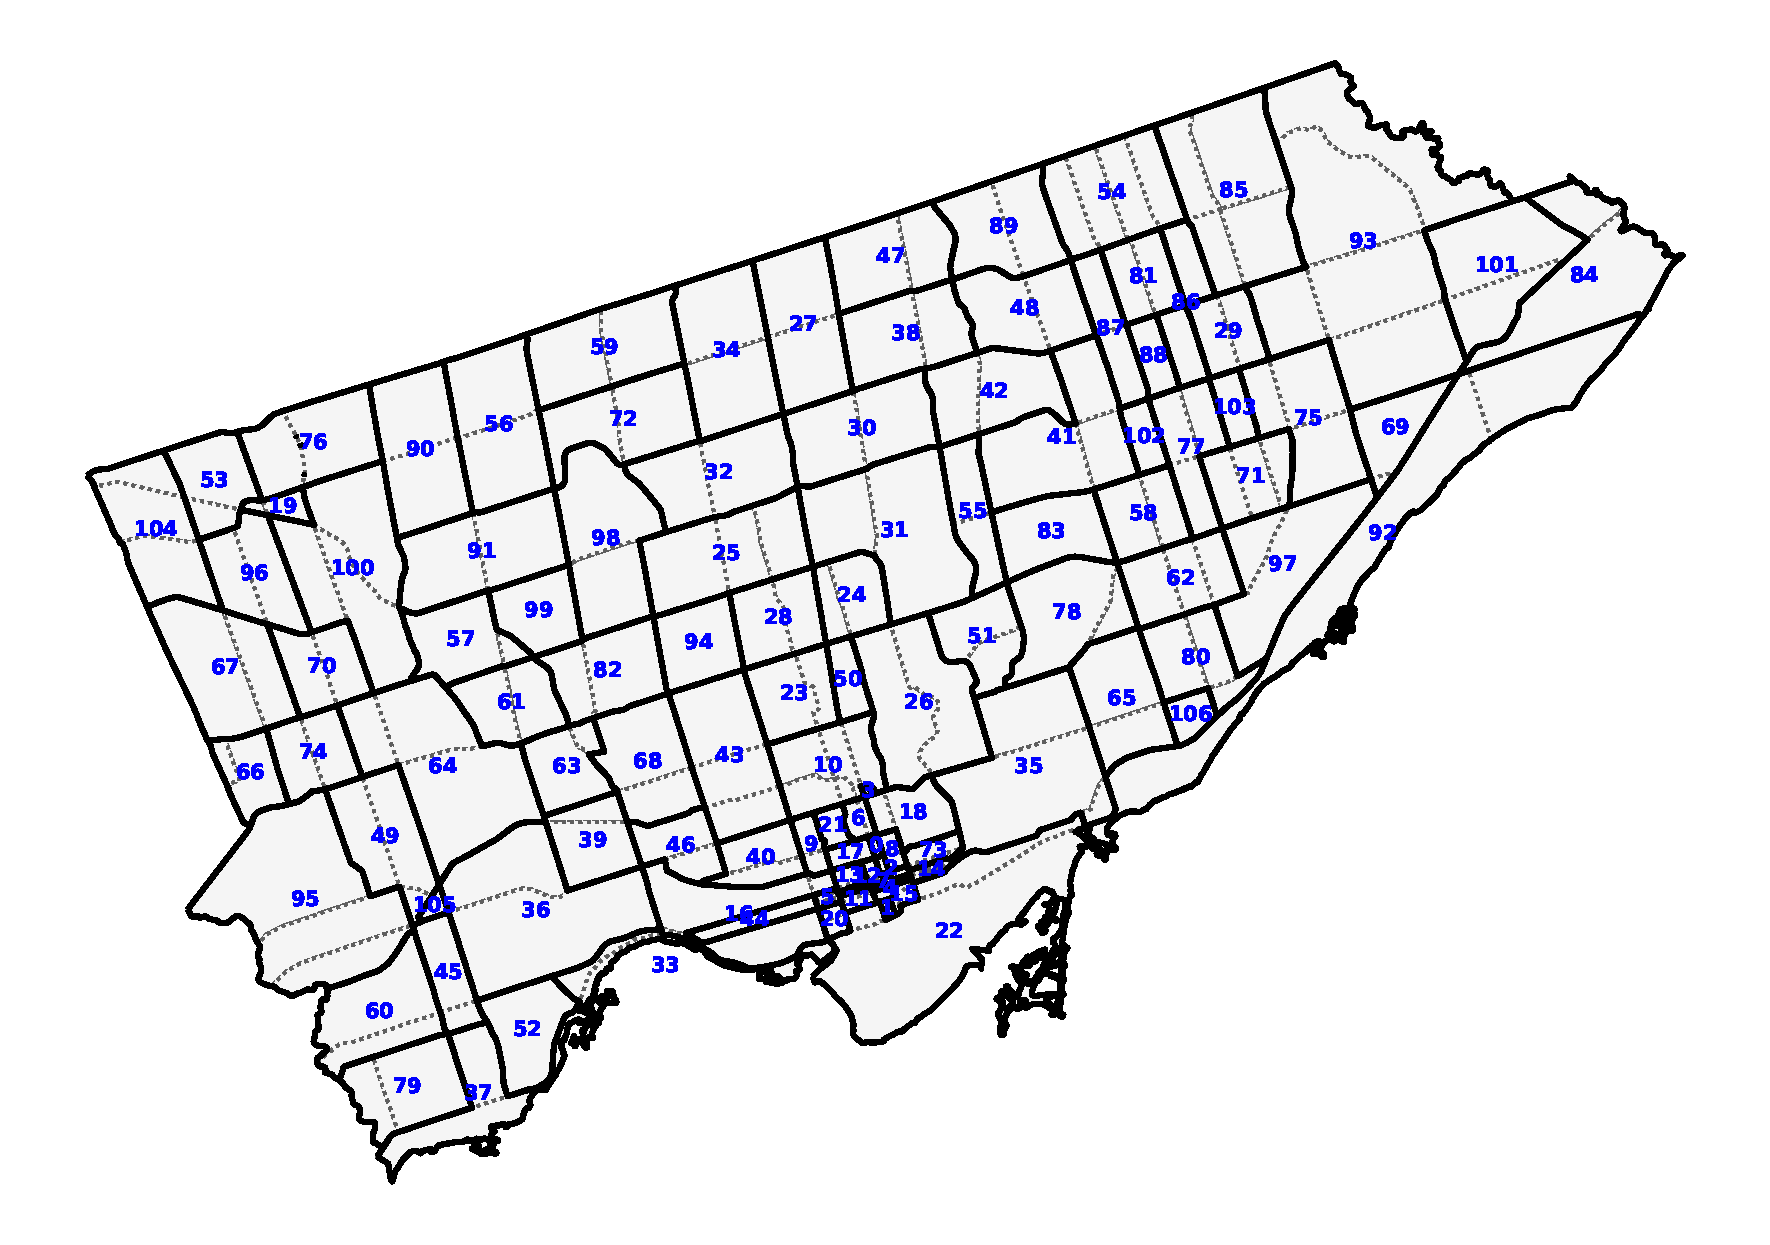
\includegraphics[width=\linewidth]{neutral_compact_clusters}
% \caption{Neutralized, shape-constrained clusters over arterial zones.}
% \label{fig:clusters_map}
% \end{figure}

\begin{figure*}[t]
\centering

\begin{subfigure}[t]{0.49\textwidth}
    \centering
    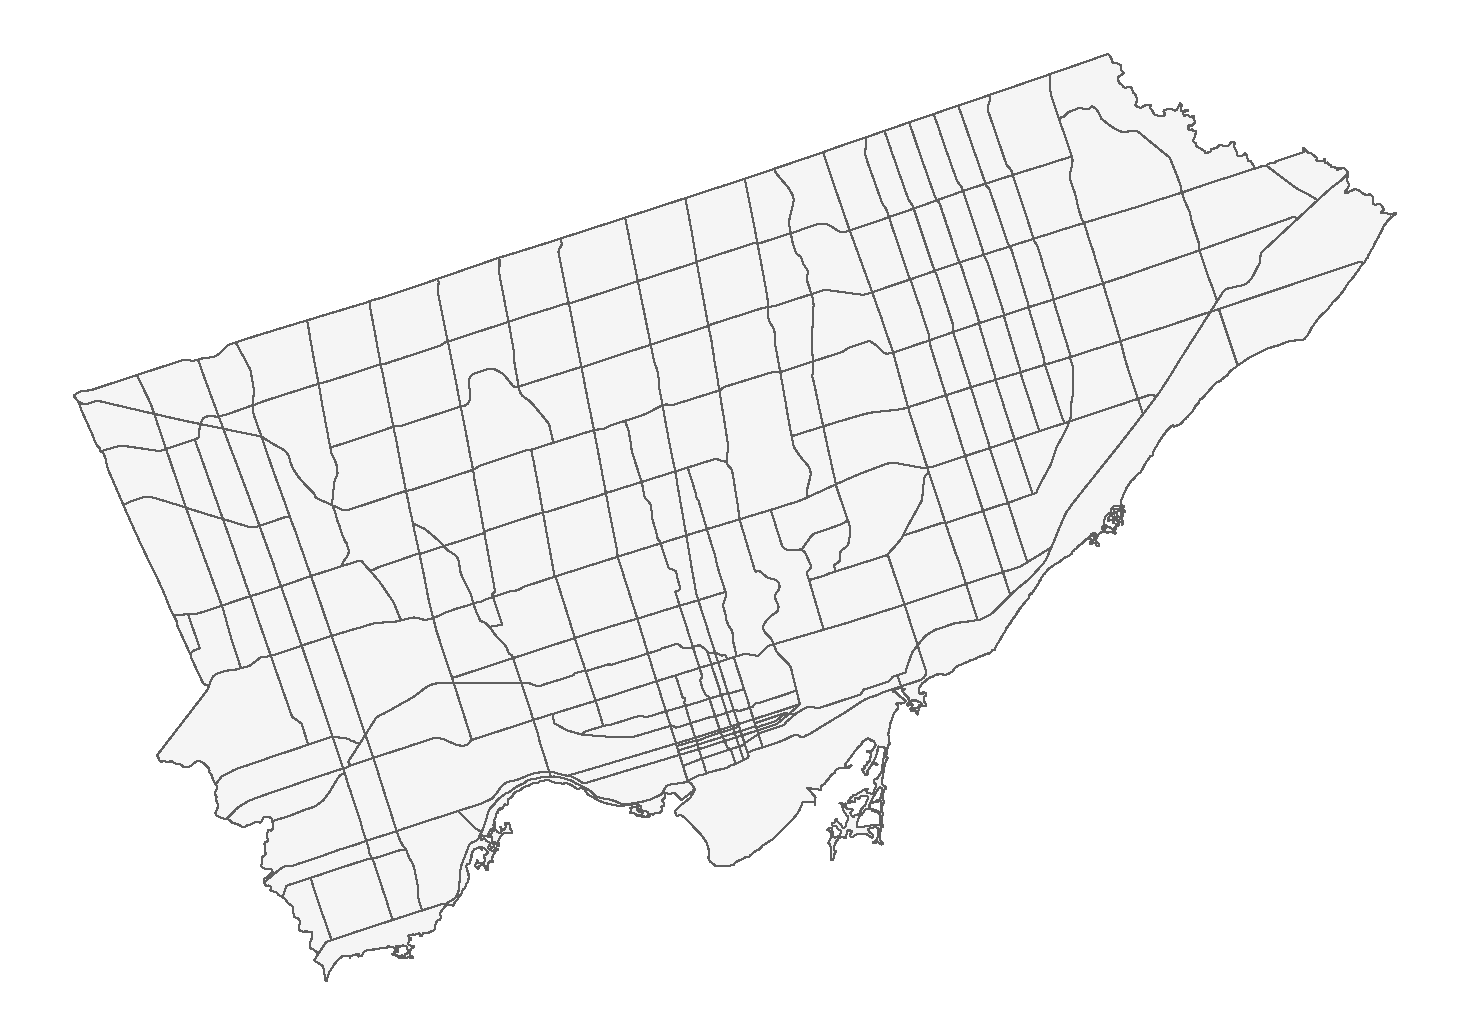
\includegraphics[width=\linewidth]{before_clustering_zones.pdf}
    \caption{Original arterial zones.}
    \label{fig:before_clusters}
\end{subfigure}
\hfill
\begin{subfigure}[t]{0.49\textwidth}
    \centering
    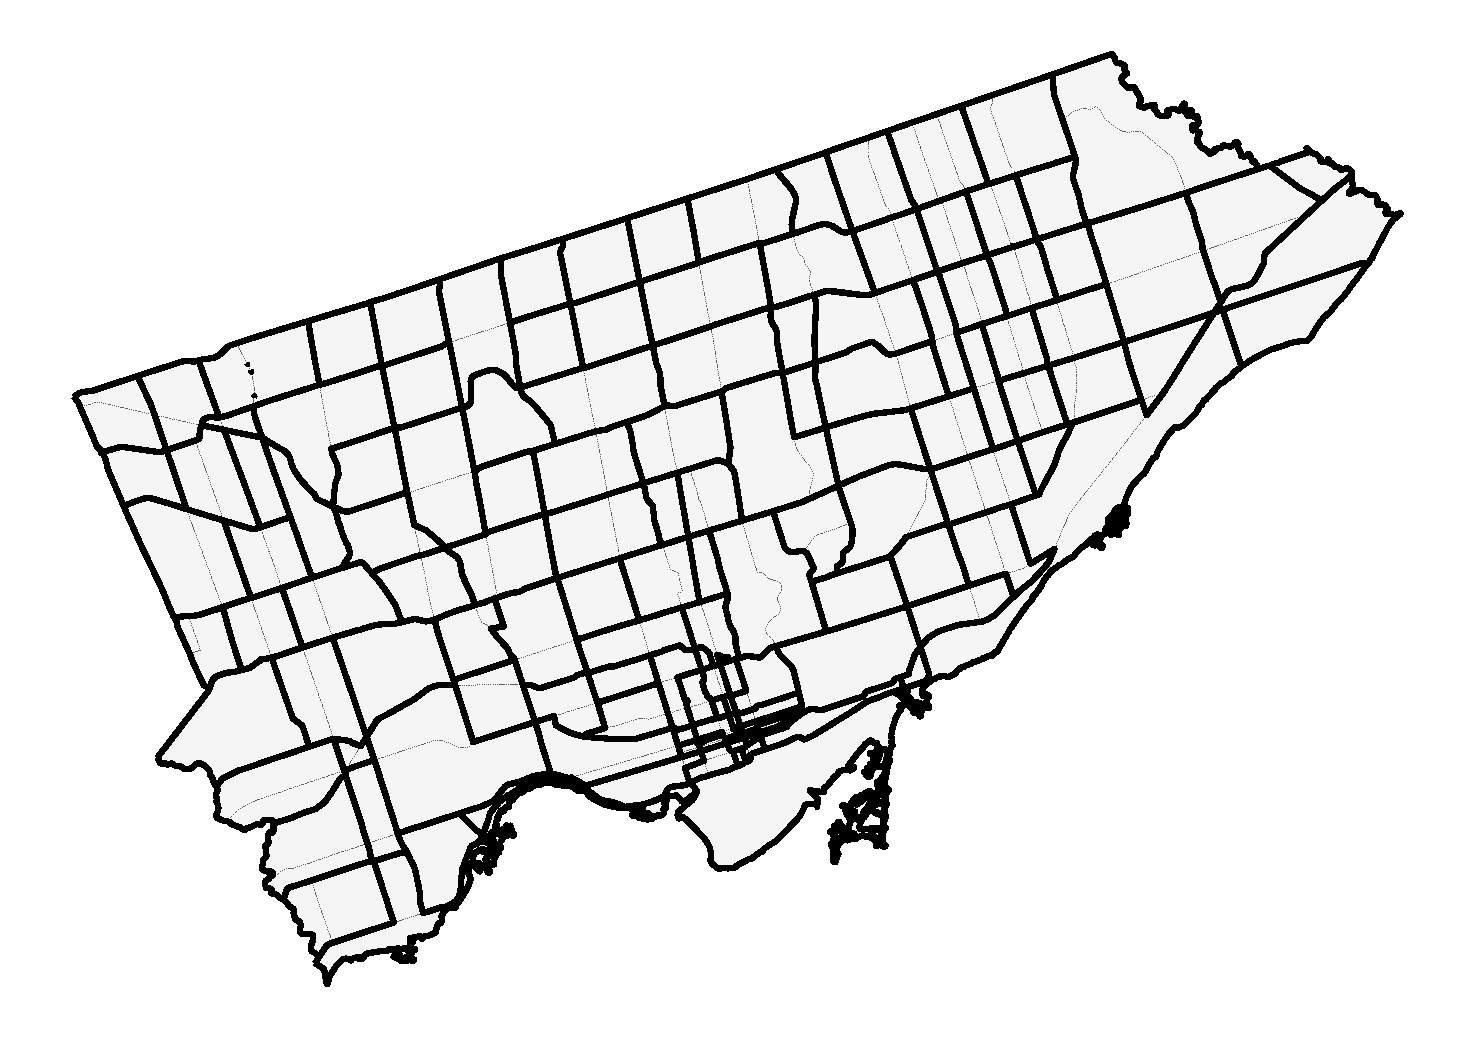
\includegraphics[width=\linewidth]{after_clustering_clusters.pdf}
    \caption{Neutralized and shape-constrained clusters.}
    \label{fig:after_clusters}
\end{subfigure}

\caption{Comparison of spatial structure before and after neutralization-based clustering.}
\label{fig:clusters_borders}
\end{figure*}
\subsection{Neutralization Improvement}

Table~\ref{tab:zone_vs_cluster_imbalance} compares the distribution of the
neutralization index before and after aggregation under the selected
configuration. Cluster-level neutralization exhibits a modest but consistent
improvement relative to the original zoning. The mean imbalance index decreases
from 0.422 at the zone level to 0.394 at the cluster level, while the median
decreases from 0.385 to 0.354. 

Although the reduction is less pronounced than in more aggressively
neutralized configurations, the results indicate that NBZC still absorbs a
portion of local BEV–ABDP mismatches within contiguous regions. The minimum
imbalance decreases to zero at the cluster level, demonstrating that certain
clusters achieve complete internal compensation. The maximum imbalance remains
unchanged at 1.000, indicating that extreme structural mismatches are not
fully eliminated but are redistributed within the regional system.
The selected configuration prioritizes geometric compactness while
retaining measurable neutralization gains, producing spatial units that are
both structurally coherent and moderately self-balanced.
\begin{table}[t]
\centering
\caption{Zone-Level vs.\ Cluster-Level Neutralization}
\label{tab:zone_vs_cluster_imbalance}
\small
\begin{tabular}{lcc}
\toprule
Metric & Zone level $\eta_i$ & Cluster level $\eta_c$ \\
\midrule
Mean $\eta$   & 0.422 & 0.394 \\
Median $\eta$ & 0.385 & 0.354 \\
Min $\eta$    & 0.001 & 0.000 \\
Max $\eta$    & 1.000 & 1.000 \\
\bottomrule
\end{tabular}
\end{table}

\subsection{Topological Effects of Regionalization}
The impact of neutralization-based regionalization on structural graph
properties is evaluated by comparing the zone-level and cluster-level
adjacency graphs. The zone graph corresponds to the rook adjacency network
over the 234 arterial zones, whereas the cluster graph is constructed by
aggregating zones within each cluster and preserving inter-cluster adjacency.
As reported in Table~\ref{tab:graph_metrics}, NBZC reduces the number of nodes
from 234 to 133 while maintaining a single connected component. The system
therefore, remains globally connected after aggregation.
Several measures indicate increased structural cohesion. Graph density rises
from 0.0184 to 0.0365, transitivity increases from 0.1882 to 0.3171, and
average local clustering increases from 0.1905 to 0.3695. The total number of
triangles also increases from 112 to 143 despite the reduction in node count.
These changes indicate stronger local interconnectedness at the meso-scale.

Navigability improves concurrently. The average shortest path length decreases
from 7.44 to 5.45, and the graph diameter decreases from 18 to 13. The graph
radius also contracts from 11 to 8, indicating a more compact and efficiently
traversable regional structure. No bridges or articulation points are present
in either representation, confirming that aggregation does not introduce
single-point structural vulnerabilities.
The maximum $k$-core remains 3 in both graphs, while the size of the
$k_{\max}$-core decreases from 230 to 130 nodes, reflecting a condensed yet
preserved structural backbone. Degree assortativity shifts from mildly positive, 0.0717, to mildly negative, $-0.0683$, suggesting that clustering moderates
degree homophily and produces a more balanced inter-regional connectivity
pattern.
Figure~\ref{fig:graphs_before_after} visualizes the zone-level and cluster-level
graphs using identical styling to highlight the structural transformation
induced by NBZC.
\begin{table}[t]
\centering
\caption{Graph Metrics: Zone Graph vs.\ Cluster Graph}
\label{tab:graph_metrics}
\scriptsize
\begin{tabular}{lrr}
\toprule
Metric & Zone graph & Cluster graph \\
\midrule
Nodes ($|V|$)         & 234   & 133 \\
Edges ($|E|$)         & 502   & 320 \\
Density               & 0.0184 & 0.0365 \\
Components            & 1     & 1 \\
Deg (min/med/mean/max) & 2/4/4.29/11 & 2/5/4.81/11 \\
Leaf fraction         & 0.000 & 0.000 \\
Transitivity          & 0.1882 & 0.3171 \\
Avg local clustering  & 0.1905 & 0.3695 \\
Triangles (total)     & 112   & 143 \\
Bridges               & 0     & 0 \\
Articulation points   & 0     & 0 \\
Max $k$-core ($k_{\max}$) & 3 & 3 \\
$k_{\max}$-core size  & 230   & 130 \\
Avg shortest path     & 7.44  & 5.45 \\
Diameter / Radius     & 18/11 & 13/8 \\
Degree assortativity  & 0.0717 & -0.0683 \\
\bottomrule
\end{tabular}
\end{table}
\begin{figure*}[h]
\centering

\begin{subfigure}[h]{0.49\textwidth}
    \centering
    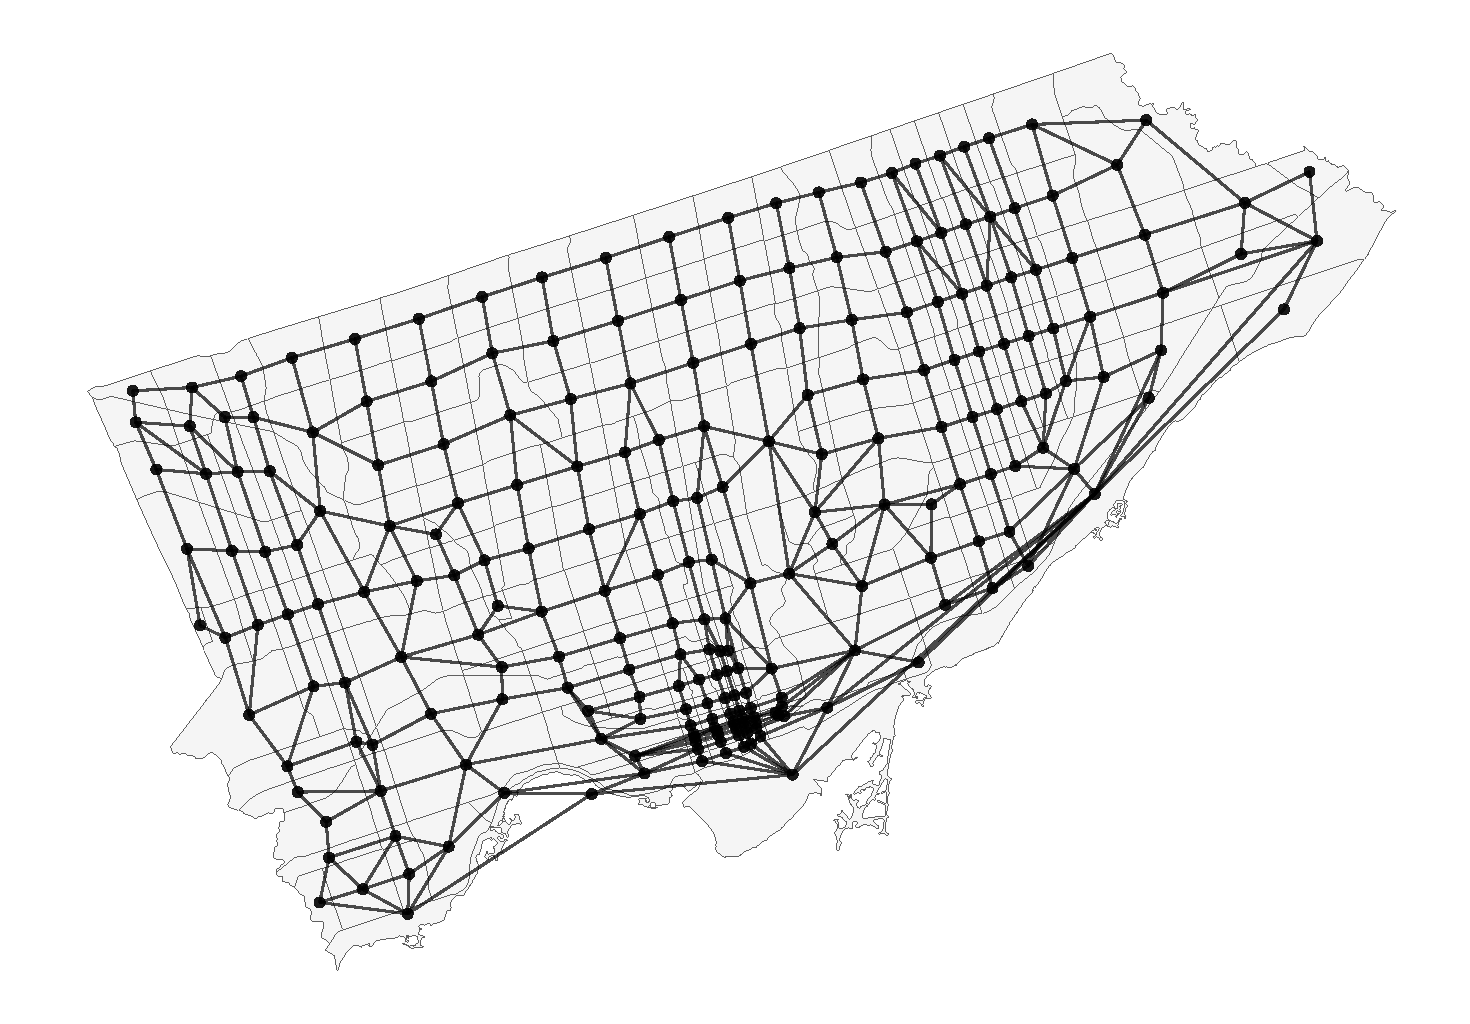
\includegraphics[width=\linewidth]{before_zone_graph.pdf}
    \caption{Zone-level adjacency graph before clustering.}
    \label{fig:graph_before}
\end{subfigure}
\hfill
\begin{subfigure}[h]{0.49\textwidth}
    \centering
    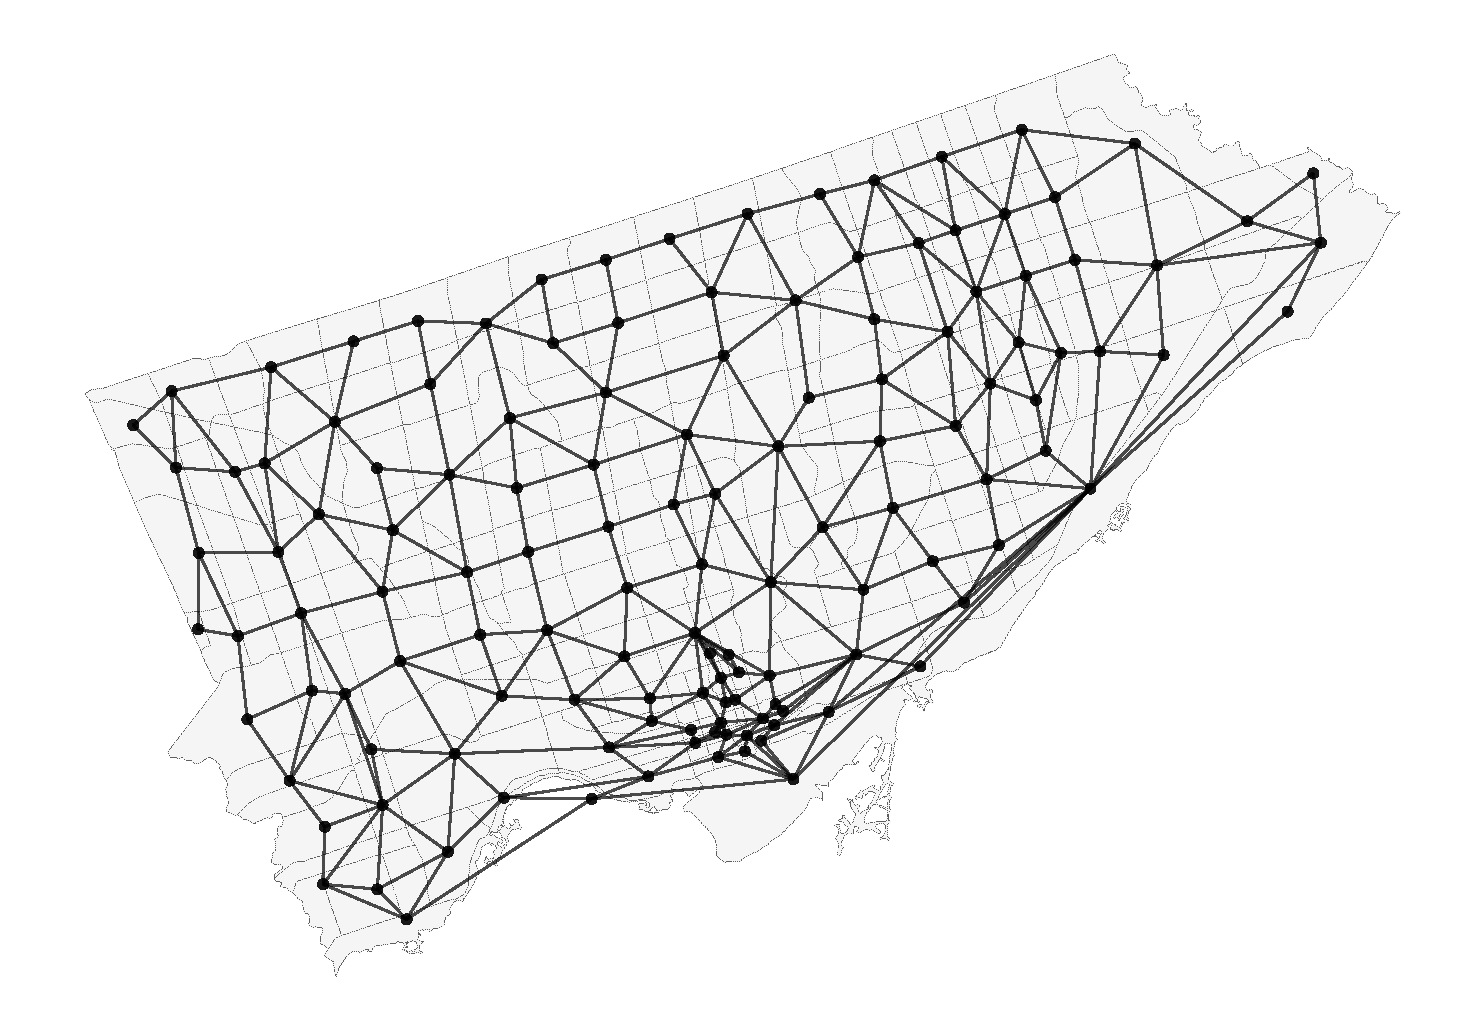
\includegraphics[width=\linewidth]{after_cluster_graph.pdf}
    \caption{Cluster-level adjacency graph after neutralization-based clustering.}
    \label{fig:graph_after}
\end{subfigure}

\caption{Comparison of graph topology before and after neutralization-based clustering.}
\label{fig:graphs_before_after}
\end{figure*}
\section{Discussion}

The results demonstrate that neutralization-based clustering produces
simultaneous improvements in behavioral balance and structural topology.
Table~\ref{tab:zone_vs_cluster_imbalance} shows that aggregation reduces
systematic imbalance between ABDP and EV density at the planning-unit
level. The mean neutralization index decreases from 0.423 at the zone
level to 0.348 at the cluster level (a 17.7\% reduction), while the
median drops more substantially from 0.398 to 0.267 (a 32.9\% reduction).
This indicates that imbalance reduction is not driven solely by extreme
zones but reflects a broad-based improvement across the distribution.
Importantly, the maximum imbalance also decreases (1.000 to 0.957),
confirming that clustering does not introduce new structural extremes.
Overall, clusters are measurably more internally self-consistent than
individual arterial zones.

Structural improvements are equally evident in the graph topology
(Table~\ref{tab:graph_metrics}). Although the number of spatial units
is reduced from 234 zones to 109 clusters (a 53\% compression), the
network remains fully connected (one component) and introduces no
bridges or articulation points. This confirms that aggregation does not
create structural fragility in the arterial backbone.

Graph cohesion increases substantially after clustering. Density more
than doubles (0.0184 to 0.0455), transitivity rises from 0.1882 to
0.3392, and average local clustering increases from 0.1905 to 0.4246.
The increase in triangle count (112 to 134) despite node reduction
further indicates stronger local interconnectedness. These changes
suggest that clusters form more cohesive corridor-scale regions rather
than loosely connected chains.

At the same time, navigability improves. The average shortest path
length decreases from 7.44 to 4.71, and the graph diameter shrinks
from 18 to 11. This reflects a more compact meso-scale topology,
reducing effective spatial distance between planning units. The
maximum $k$-core remains 3 in both cases, indicating that clustering
preserves the fundamental hierarchical backbone of the arterial system
while simplifying its surface complexity.

Taken together, the two tables demonstrate that NBZC achieves a dual
improvement: behavioral neutralization and structural consolidation.
Clusters are not only more internally balanced in terms of BEV–ABDP
alignment, but they also form a denser, more cohesive, and more
navigable spatial graph without sacrificing global connectivity.
This confirms that neutralization-based regionalization enhances
planning stability while preserving the integrity of the urban
arterial network.

\section{Results: Emergent Planning District Structure}
\subsection{Community Detection Parameter Sweep and Experimental Design}

To derive robust planning districts, we conducted a systematic
parameter sweep across multiple community detection algorithms.
Each candidate partition was evaluated using the neutralization
objective $J_{\mathrm{ne}}$.
The connected component considered in this stage consisted of 133 clustered nodes derived from the previous neutralization step. To systematically explore the meso-scale structure of the graph, multiple community detection algorithms were evaluated under comprehensive parameter sweeps. For methods requiring a predefined number of communities, the community count was varied over the range $k \in \{2, \dots, 130\}$, resulting in 130 admissible values. To account for stochastic variability in randomized algorithms, each configuration was repeated over 20 independent random seeds. For the Louvain method, six resolution parameters $\gamma \in \{0.3, 0.5, 0.7, 1.0, 1.5, 2.0\}$ were examined to capture multi-scale modular structures. Additionally, the Girvan-Newman hierarchical procedure was executed for 15 successive split levels to evaluate progressively finer community decompositions. The applied community extraction methods included greedy modularity maximization, label propagation, asynchronous fluid communities, Kernighan-Lin bisection, Louvain resolution sweeping, and the Girvan--Newman hierarchy. In total, 2,776 candidate partitions were generated and evaluated. For each community count $k \in \{2, \dots, 130\}$, the partition attaining the minimum $J_{\mathrm{ne}}$ across all algorithms and parameter configurations was selected, yielding the best achievable neutralization performance at each structural resolution.
As shown in Fig.~4, the curve relating the number of communities $k$ to the corresponding best-achievable $J_{\mathrm{ne}}$ exhibits a generally increasing trend as $k$ grows. The neutralization objective is lowest for coarse partitions and progressively increases as the graph is fragmented into finer districts. This behavior indicates that excessive subdivision reduces the capacity of districts to internally balance demand and activity signals, thereby degrading behavioral self-sufficiency. 
% The visible elbow around $k \approx 47$ marks a structural transition in the rate of degradation, suggesting a meso-scale resolution beyond which further fragmentation yields diminishing structural benefits while increasing neutralization cost.
\begin{figure}[!h]
\centering
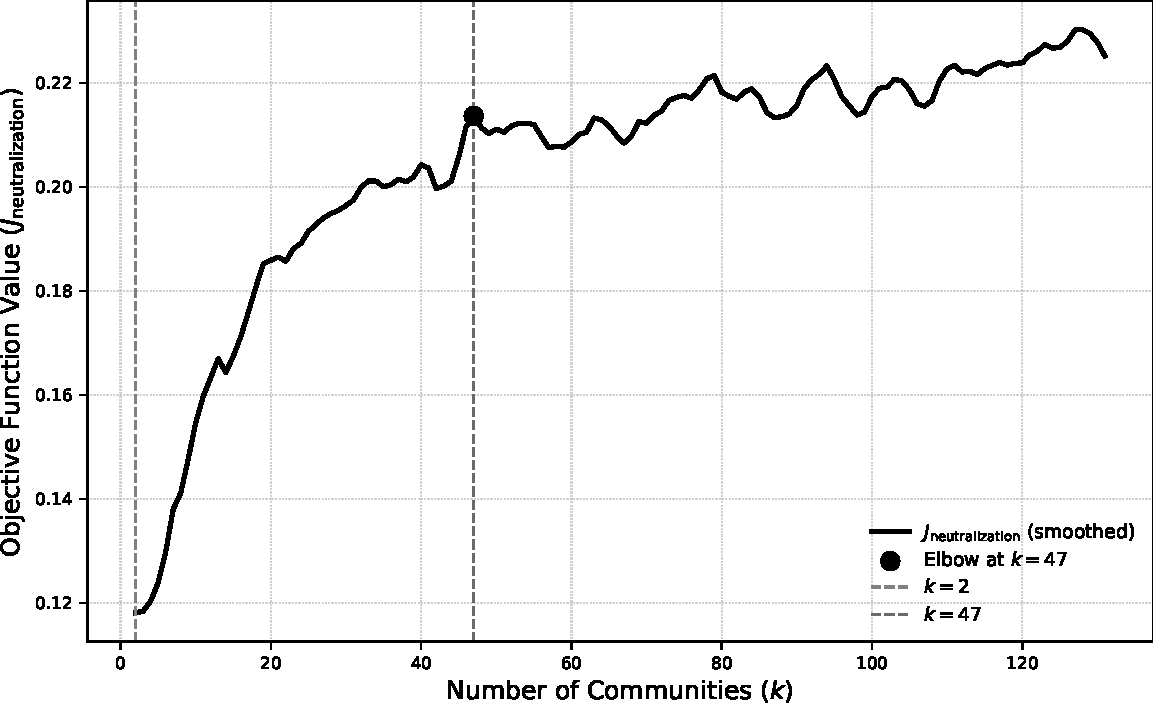
\includegraphics[width=\columnwidth]{communities and neutrilization knee_curve (1).pdf}
\caption{The minimum objective value across all algorithms and parameter configurations.}
\label{fig:best_J_vs_k}
\end{figure}
Curvature analysis of $J_{\text{best}}(k)$ revealed a structural transition
in the growth behavior of the neutralization objective. An knee was detected
at $k^\star = 47$, marking the point at which the increase in
$J_{\mathrm{ne}}$ transitions from a steeper growth regime
to a relatively stable, slowly varying regime.
Beyond this transition point, the marginal increase in the neutralization
objective remains comparatively small, indicating that further subdivision
does not substantially alter the behavioral balance. This suggests that
community counts near $k^\star$ represent a meso-scale structural resolution
at which the system transitions from coarse aggregation to a stabilized
behavioral regime without significant additional fragmentation cost.
\subsection{Structural Pareto Front}

Within the admissible window, all candidate partitions were evaluated 
using coverage, modularity, and performance. Pareto filtering produced a 
set $\mathcal{P}^\star$ of non-dominated structural configurations. 
Subsequent behavioral restriction retained only those partitions within 
the lowest $\rho$-quantile of $J_{\text{neutral}}$, forming 
$\mathcal{P}^\star_\rho$.

The resulting Pareto-efficient solutions demonstrated the following ranges:

\begin{align}
\mathrm{Coverage} &\in [\cdot,\cdot], \\
Q &\in [\cdot,\cdot], \\
\mathrm{Performance} &\in [\cdot,\cdot], \\
J_{\text{neutral}} &\in [\cdot,\cdot].
\end{align}

These values confirm that strong structural coherence can be achieved 
without sacrificing behavioral balance.

\subsection{Final District Selection}

Applying the lexicographic maximization rule defined in 
(\ref{eq:final_selection_lex}), the optimal planning district partition 
$\mathcal{G}^\star$ was selected.

The selected configuration corresponds to:

\begin{equation}
k^\star = |\mathcal{G}^\star|,
\end{equation}

with structural metrics:

\begin{align}
Q(\mathcal{G}^\star) &= \cdot, \\
\mathrm{Coverage}(\mathcal{G}^\star) &= \cdot, \\
\mathrm{Performance}(\mathcal{G}^\star) &= \cdot,
\end{align}

and behavioral balance:

\begin{equation}
J_{\text{neutral}}(\mathcal{G}^\star) = \cdot.
\end{equation}

Notably, $k^\star$ lies strictly within the stability window, confirming 
that the selected district scale emerges from the interaction between 
behavioral neutralization dynamics and graph structural coherence rather 
than from arbitrary policy assumptions.

\subsection{Spatial Interpretation}

The resulting planning districts exhibit contiguous and compact spatial 
structure, reflecting the underlying cluster adjacency network. 
Communities are spatially coherent and display balanced internal dwell 
capacity relative to EV demand intensity. Regions with high 
activity-driven dwell potential are co-located with elevated EV density, 
resulting in low values of $\eta_g$ across districts.

The selected configuration avoids both over-aggregation (which would mask 
intra-urban heterogeneity) and over-fragmentation (which would degrade 
behavioral self-sufficiency). This confirms that the integrated 
behavioral–structural framework successfully identifies a meso-scale 
district system aligned with both urban activity patterns and network 
topology.

\subsection{Implications for Planning}

The results demonstrate that planning district scale is not arbitrary but 
emerges from measurable structural–behavioral interactions. 
Pure modularity maximization would favor finer partitions with higher 
structural separation but degraded behavioral neutrality. Conversely, 
pure neutralization minimization would favor coarse partitions that lack 
structural discrimination. 

The proposed Pareto-constrained selection balances these competing forces, 
yielding planning districts that are:

\begin{itemize}
\item Behaviorally self-balanced,
\item Structurally cohesive,
\item Spatially contiguous,
\item Policy-relevant at the meso-scale.
\end{itemize}

This confirms the validity of the methodology introduced in Section~III.
% =========================
% 9. Conclusion
% =========================
\section{Conclusion}
This paper presented a behavioral-to-structural framework for urban EV
fast-charging planning that links dwell feasibility to meso-scale
regionalization. We first introduced an ABDP
metric that converts POI composition into a continuous dwell-compatibility
signal aligned with fast-charging session durations. We then proposed
NBZC, which aggregates arterial zones
into contiguous and compact corridor regions while approximately neutralizing the mismatch between normalized ABDP and normalized EV density.

Beyond improving fit between behavioral feasibility and mobility intensity,
neutralization has a direct planning interpretation: it increases the \emph{self-sufficiency} of meso-scale planning units. Regions with large
aggregate imbalance must rely on cross-boundary behavioral flows either by attracting EV demand from adjacent regions when the dwell capacity exceeds the EV
presence, or by exporting charging behavior outward when EV intensity exceeds dwell compatibility. Such spillover dependence increases sensitivity to
boundary definitions, localized anomalies, and temporal shifts in activity and
travel patterns, thereby increasing uncertainty in long-horizon allocation and
grid coordination. By internalizing opposing zone-level deviations within each
region, NBZC reduces cross-boundary dependence and yields corridor-scale units
whose charging feasibility is supported more consistently from within the
region.

In the Toronto case study, NBZC produced corridor-aligned regions that reduce
cluster-level imbalance while preserving global connectivity and strengthening graph cohesion. These results suggest that ABDP can serve as a transferable
behavioral screening signal and that neutralization-based regionalization can
provide more stable, interpretable, and planning-relevant units for long-term
fast-charging deployment. Future work will integrate the proposed regions into
downstream capacity allocation and grid-aware optimization, and evaluate
robustness under temporal variation in activity patterns and EV adoption. \cite{Annan2024}\cite{Katontoka2025}\cite{Zhang2025}\cite{Wang2023}\cite{Sun2024}\cite{Matkovic2024}\cite{Qin2026}\cite{Yuan2025}\cite{WANG_DENG_YAN_LI_2025}\cite{Zechao2024}


% =========================
% References
% =========================
\bibliographystyle{IEEEtran}
\bibliography{references} % put your BibTeX entries in references.bib


% \balance % uncomment if last page columns are uneven
\end{document}